\documentclass[a4paper]{article}
%\documentclass[a4paper]{scrbook}


% definitions
\def\D{\partial}
\def\a{\alpha}
\def\dd{\displaystyle}
\def\ke{{k- \varepsilon}}
\def\e{\varepsilon}
\def\12{{\frac{1}{2}}}
\def\e{\varepsilon}
\def\ub{\bar{u}}
\def\vb{\bar{v}}
\def\pb{\bar{p}}
\def\sij{\bar{S_{ij}}}
\def\vij{\overline{v'_iv'_j}}
\def\vik{\overline{v'_iv'_k}}
\def\vjk{\overline{v'_jv'_k}}
\def\uv{\overline{v'_1v'_2}}
\def\vw{\overline{v'_2v'_3}}
\def\uw{\overline{v'_1v'_3}}
\def\uu{\overline{v_1^{\prime 2}}}
\def\vv{\overline{v_2^{\prime 2}}}
\def\ww{\overline{v_3^{\prime 2}}}

\usepackage[colorlinks=true,linkcolor=blue,anchorcolor=blue,urlcolor=blue,citecolor=blue]{hyperref}


\def\solidline{{$\textcolor{blue}{\overline{\hskip 0.5cm}}\ $}}
\def\dashedline{{$\textcolor{red}{\overline{\hskip 0.1cm}\ \overline{\hskip 0.1cm}\ \overline{\hskip 0.1cm}\ }$}}
\def\dashdottedline{$\overline{\hskip 0.1cm}\ \overline{\hskip 0.03cm}\ \overline{\hskip 0.1cm}\ $}
\def\dottedline{$\overline{\hskip 0.04cm}\ \overline{\hskip 0.04cm}\ \overline{\hskip 0.04cm}\ $}




%\setlength{\headheight}{ 27.8pt}
\usepackage{color}
\usepackage{subfigure}
\usepackage{graphicx,psfrag}
\usepackage{amsmath}
\usepackage{amsfonts}
\usepackage{latexsym}
\usepackage{amssymb}
\usepackage[outdir=./]{epstopdf}
\usepackage{grffile}
%\usepackage{\mathaccent}


\def\karm{von  K\'arm\'an }

\pagestyle{myheadings}
\renewcommand{\subsectionmark}[1]{\markright{\thesubsection. #1}}
\renewcommand{\sectionmark}[1]{\markright{\thesection. #1}}


\begin{document}


%\title{MTF065 Turbulent Flow: An Example of a Report}
\title{Turbulent channel flow tests}
%\author{L. Davidson \\
%Division of Fluid Dynamics,
%Department of Applied Mechanics\\
%Chalmers University of Technology, G\"oteborg, Sweden\\
%\href{http://www.tfd.chalmers.se/\textasciitilde lada/}
%{\tt http://www.tfd.chalmers.se/\textasciitilde lada/}\\
%}

\maketitle

\cleardoublepage
\newpage
%\section*{Channel Flow tests}
%
%The idea for this investigation is to check the cause for non-existant eddy viscosity in the channel for the ${Re_{\tau}} = 395$.
%We would perform two set of simulations on the mesh resolution 192x64x96 (Mesh1). We would write out all the quantities i.e. gradients $\frac{\D v_i}{\D x_i}$ , strain rates contraction and the traceless tensor formulated with the square of the velocity gradient tensor. In short, it would be same as we did previously in the poiseuille flow simulations and the Taylor green vortex simulations. \\

%{\bf i. Mesh 1 AA2016Wale}. We will perform the simulation for total 300,000 time steps and write out the data only for the $300,000^{th}$ time-step. In this tests we will not perform any kind of averaging, but write out all the details as discussed above. The idea here is to observe the order for the different quantities written out and to estimate the orgin of the error.\\
%
%{\bf ii. Mesh 1 AA2016Wale -  smaller perturbation number ($\epsilon$)}. Here we will perform the same simulation as above, but with the smaller $\epsilon$ added to make the system well-poised.
%The definition of which is as follows:\\
%%
%\begin{equation}
%\label{eddy-viscosity}
%\begin{split}
%{\nu_t} &= \left({C_w}{\Delta}\right)^{2}
%\frac{\left({S_{ij}^{d}}{S_{ij}^{d}}\right)^{3/2}}{\left(\sij \sij\right)^{5/2} + {\left({S_{ij}^{d}}{S_{ij}^{d}}\right)^{5/4}} + \epsilon}
%\end{split}
%\end{equation}
%%
%\\
%where, $\epsilon$ in our case is of the order $\sim 10^{-8}$.\\
%
%In this simulation we will change the value of $\epsilon$ to $\sim 10^{-30}$ or lower as the order of the terms in the numerator and the denominator are in between $\sim 10^{-18}$ to $\sim 10^{-25}$. Adding the epsilon of $\sim 10^{-8}$ in the denominator, which is relatively a larger number, is the reason we do not see the eddy viscosity in the channel. The purpose of this test is to see if we get the same orders of magnitude of the eddy viscosity as obtained in the tests performed using Matlab.
%\subsection{Discussion $9^{th}$ May}
%
%{\bf I. Test 1}. Here we have to improve the conditioning for the eddy viscosity in a more general way, rather than adding a constant  approximately. The idea as discussed by professor is as follows:
%\begin{equation}
%\label{eddy-viscosity-conditioning}
%\begin{split}
%A^{3/2} &= \left({S_{ij}^{d}}{S_{ij}^{d}}\right)^{3/2},\\
%A^{5/4} &= \left({S_{ij}^{d}}{S_{ij}^{d}}\right)^{5/4},\\
%B^{5/2} &= \left(\sij \sij\right)^{5/2}
%\end{split}
%\end{equation}
%When terms of the equation ~\ref{eddy-viscosity-conditioning} are replaced in the equation for ~\ref{eddy-viscosity} it looks as follows (not considering $\epsilon$ now):
%\begin{equation}
%\label{eddy-viscosity-changed}
%\begin{split}\\
%{\nu_t} &= \left({C_w}{\Delta}\right)^{2}
%\frac{A^{3/2}}{B^{5/2} + {A^{5/4}}},\\
%{OP} &= \frac{A^{3/2}}{B^{5/2} + {A^{5/4}}}\\
%\end{split}
%\end{equation}\\
%Now in the equation ~\ref{eddy-viscosity-changed} let's divide by ${A^{5/4}}$ and ${OP}$ would like:
%\begin{equation}
%\label{some_modification}
%\begin{split}\\
%{OP} &= \frac{A^{3/2}A^{\--5/4}}{\left(B^{5/2}\// {A^{5/4}}\right) + 1}\\
%\end{split}
%\end{equation}\\
%Some sort of this modification can give a general conditioning of the eddy viscosity.\\
%{\bf II. Channel flow}.  Pressure and the density are negative i.e. mass deficit in the channel\\
%{\bf III. Taylor green vortex}. Finer resolution with changed value of $\epsilon$. %%
%\begin{equation}
%\label{some_modification}
%\begin{split}
%{OP} &= \frac{A^{1/4}}{\left(B^{1/2}\// {\left(A^{1/4} + 10^{-10}\right)}\right)^{5} + 1}
%\end{split}
%\end{equation}\\
%%Some sort of this modification can give a general conditioning of the eddy viscosity.\\
%%{\bf II. Channel flow}.  Pressure and the density are negative i.e. mass deficit in the channel\\
%%{\bf III. Taylor green vortex}. Finer resolution with changed value of $\epsilon$. 
%
%\subsection{Next steps $15^{th} May$}
%
%Since the reason for the missing eddy viscosity is found, $\epsilon$ = $10^{-30}$, and an appropriate wale model co-efficient, $C_{W} = 0.55$, we should start the wale model simulations on the channel flow.
%\\
%\\
%{\bf i}. AA2016Wale and OneWale\\
%{\bf ii}. AA2016wale with double precision. This will be a comparison to see if any significant changes are present in the flow.
\pagenumbering{roman}

\newpage
\tableofcontents

\input{01_Channel_flow_test/Channel_flow_test}

\newpage

\section{Results and discussion}

\newpage

\section{Introduction Turbulence modelling}

{\bf i DNS}.\\
Direct numerical simulation (DNS) method uses a modelling-free approach for approximation of the exact solution, as the navier-stokes equation comprises of all turbulence mechanisms. Since the turbulence is three dimensional and inherently instationary it has to take in to account all the components present in the navier stokes equation.Turbulence involves the interaction in between the scales of various different sizes and thus to represnt the exact solution or the characteristics of the turbulent flow considered correctly, the DNS method emphasises on the fine spatial and temporal resolution of the meshes. Apart from that this method requires the discretization methods to have low level of numerical dissipation and dispersion. In order to correctly determine the effects of the turbulence intensity, the fluctuating flow variables which satisfy the navier stokes equation are provided as inputs.
\\
{\bf ii DES}.\\
Detached eddy simulation, DES, combines the approach of RANS and the LES method; it therefore belongs to the class of the hybrid RANS-LES simulations. The basic idea of this method is that the near wall boundary layer would be resolved using the RANS approach, while the usuage of LES to (correctly) resolve such regions requires a very fine spatial and temporal resolution, as the turbulent scales to be resolved in the boundary layers are very small. On the other hand, the detached regions, wakes and the free shear layers are the regions, where the RANS model frequently fails, are handled by the LES.\\
\\
 DES was first introduced by {\it Spalart et al.}. The goal was to compute the aerodynamic flows involving massive seperation with a moderate increase in the grid resolution compared to the RANS method. The idea behind the DES is to segregate the flow, using suitable detectors, in to the domains where the entire energy spectrum will be modelled using the RANS (near wall boundary layer) or the large energy containing structures are resolved using the LES method (detached flow region). Therefore in this approach, a suitable method is chosen, for each domain, in terms of efficiency and accuracy.\\
\\
In comparison with LES, for the computation of the flows involving the boundary layer, DES reduces the computational effort significantly. Since the flows involved are unsteady and three dimensional turbulent flows, the computational effort will be relatively higher when compared with RANS.\\
\\
Avery good compilation of the hybrid RANS-LES approach is found in {\it Fröhlich and von Tersi (2008)}\\


\begin{equation}
\label{eddy-viscosity-conditioning}
\begin{split}
A^{3/2} &= \left({S_{ij}^{d}}{S_{ij}^{d}}\right)^{3/2},\\ A^{5/4} &= \left({S_{ij}^{d}}{S_{ij}^{d}}\right)^{5/4},\\ B^{5/2} &= \left(\sij \sij\right)^{5/2}\\
\end{split}
\end{equation}
When terms of the equation ~\ref{eddy-viscosity-conditioning} are replaced in the equation for ~\ref{eddy-viscosity} it looks as follows (not considering $\epsilon$ now):
\begin{equation}
\label{eddy-viscosity-changed}
\begin{split}\\
{\nu_t} &= \left({C_w}{\Delta}\right)^{2}
\frac{A^{3/2}}{B^{5/2} + {A^{5/4}}},\\
{OP} &= \frac{A^{3/2}}{B^{5/2} + {A^{5/4}}}\\
\end{split}
\end{equation}\\
Now in the equation ~\ref{eddy-viscosity-changed} let's divide by ${A^{5/4}}$ and ${OP}$ would like:
\begin{equation}
\label{some_modification}
\begin{split}\\
{OP} &= \frac{A^{3/2}A^{\--5/4}}{\left(B^{5/2}\// {A^{5/4}}\right) + 1}\\
\end{split}
\end{equation}\\
Some sort of this modification can give a general conditioning of the eddy viscosity.\\
{\bf II. Channel flow}.  Pressure and the density are negative i.e. mass deficit in the channel\\
{\bf III. Taylor green vortex}. Finer resolution with changed value of $\epsilon$. 

\newpage


\section{Turbulent mean flow}

There is no definition on turbulent flow, but it has a number of characteristic
features (see Pope~\cite{pope:book} and Tennekes \& Lumley~\cite{tennekes:lumley}) such as:

{\bf I. Irregularity}. Turbulent flow is irregular, random and chaotic.  The flow consists
of a spectrum of different scales (eddy sizes).
We do not have any exact definition of an \emph{turbulent eddy}\marginpar{\bf turbulent eddy}, but
we suppose that it exists in a certain region in space for a certain time and that it is subsequently
destroyed (by the cascade process or by dissipation, see below).
It has a characteristic velocity and length (called a velocity and length scale). The region
covered by a large eddy may well enclose also smaller eddies.
The largest eddies are of the order of the flow geometry (i.e. boundary layer thickness,
jet width, etc).
At the other end of the spectra we have the smallest eddies
which are dissipated by viscous forces (stresses) into thermal energy resulting in a temperature increase. Even though
turbulence is chaotic it is deterministic and is described by the Navier-Stokes equations.

 $S=1.51$, $-0.27$ and $-0.09$. The flatness
are $F= 7.68$, $5.81$ and $2.77$.


\begin{figure}[bt]
\centering
\begin{minipage}[b]{0.33\textwidth}
\psfrag{v1-2}[r][1][1][-90]{}
\psfrag{u}[r][1][1][-90]{$v'_1$}
\psfrag{t}[t][1][1][0]{$t$}
\subfigure[$S=1.51$ and $F= 7.68$]{
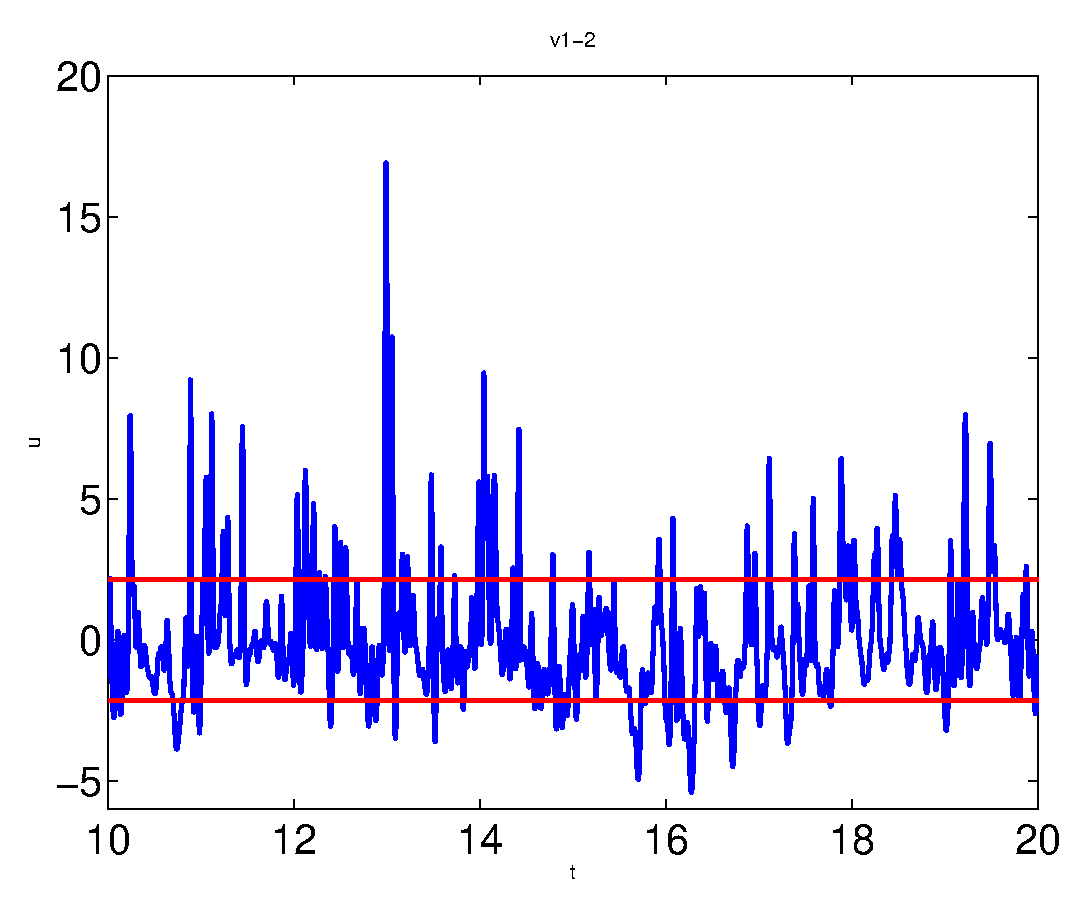
\includegraphics[width=3.8cm]{figur/v_time_2_new.eps}
%\includegraphics[width=4.0cm]{figur/AA2016_Profiles_global_coords_comparison.jpg}
%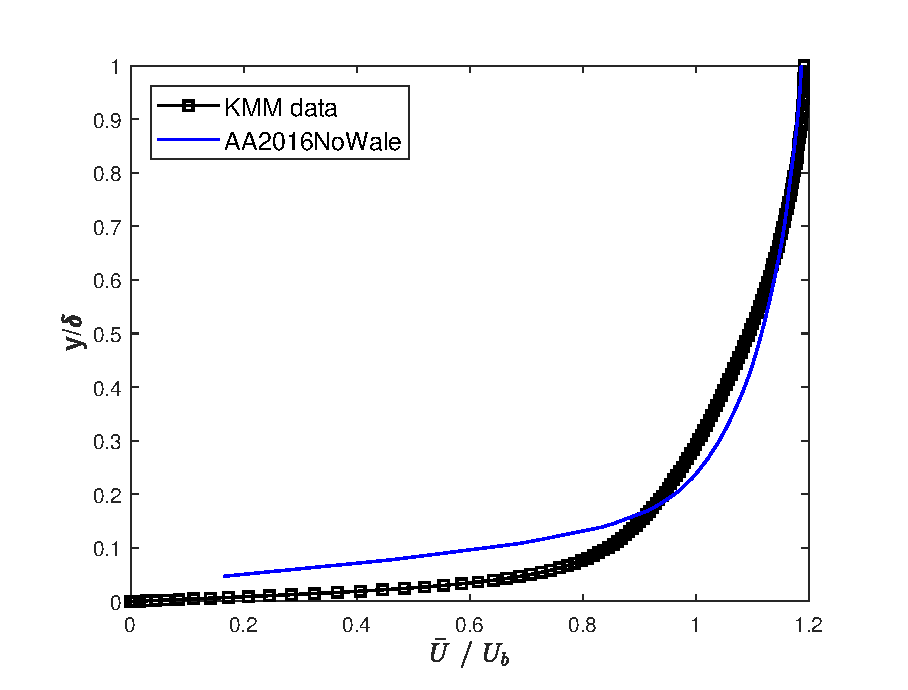
\includegraphics[width=4.0cm]{figur/AA2016_test.eps}
}
\end{minipage}%
\begin{minipage}[b]{0.33\textwidth}
\psfrag{v1-3}[r][1][1][-90]{}
\psfrag{u}[r][1][1][-90]{}
\psfrag{t}[t][1][1][0]{$t$}
\subfigure[$S=-0.27$ and $F= 5.81$]{
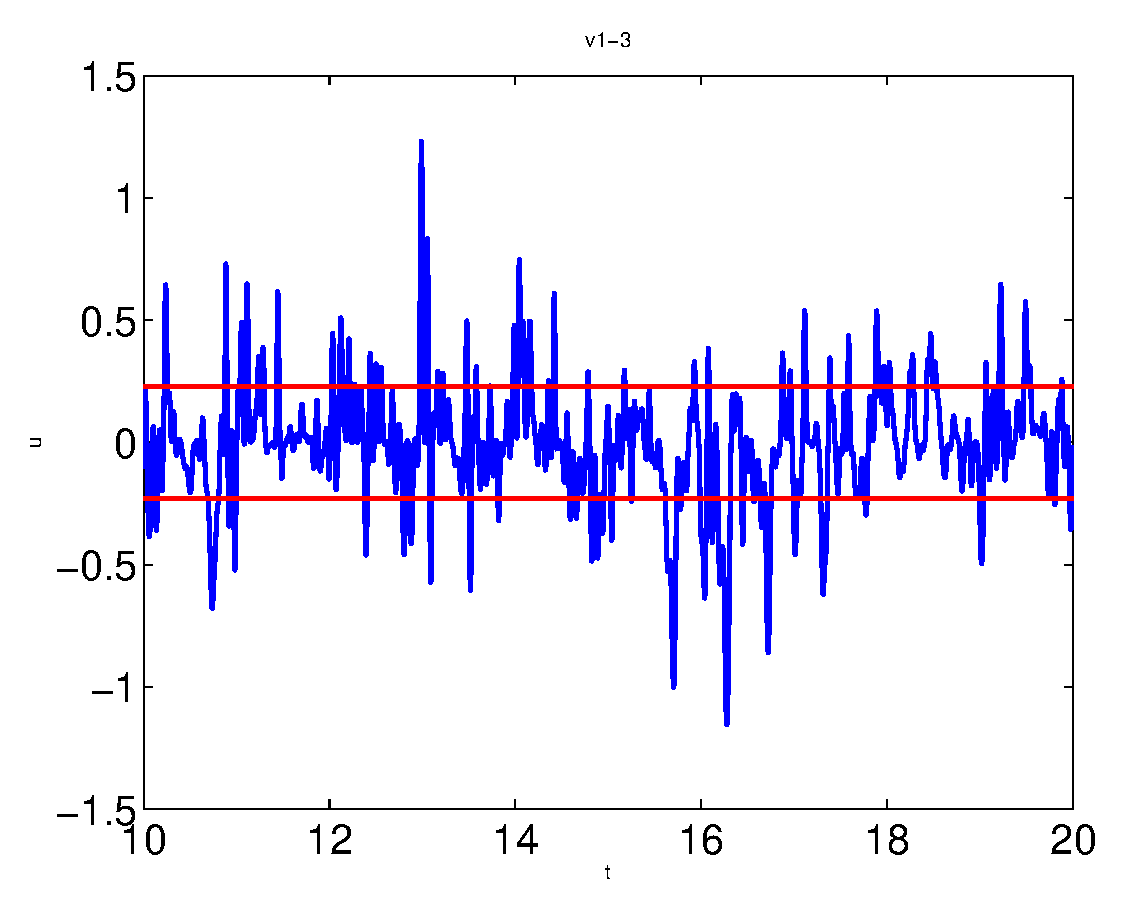
\includegraphics[width=3.8cm]{figur/v_time_3_new.eps}
}
\end{minipage}%
\begin{minipage}[b]{0.33\textwidth}
\psfrag{v1-3-low}[r][1][1][-90]{}
\psfrag{u}[r][1][1][-90]{}
\psfrag{t}[t][1][1][0]{$t$}
\subfigure[$S=-0.09$ and $F= 2.77$]{
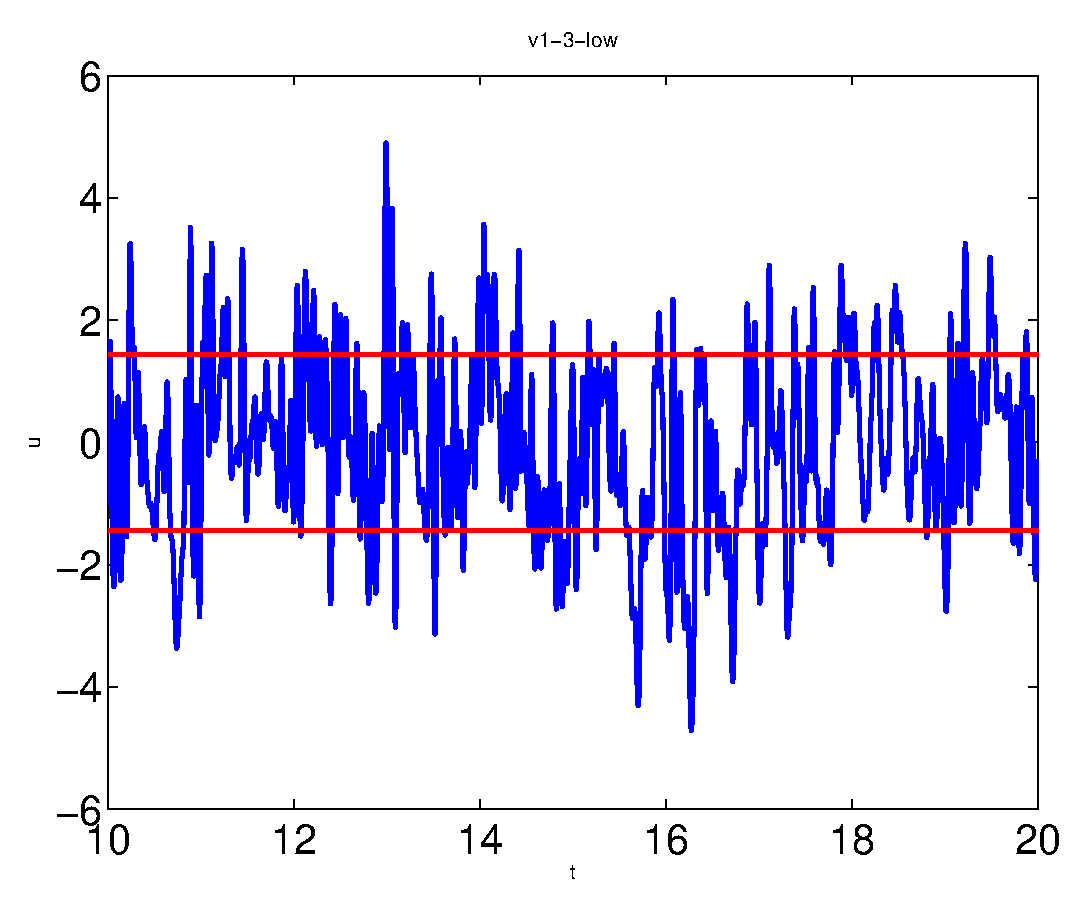
\includegraphics[width=3.8cm]{figur/v_time_3_new_low.eps}
}
\end{minipage}%
\caption{Time history of $v'_1$. Horisontal red lines show $\pm v_{1,rms}$.}
\label{time-hist}
\end{figure}


Consider the  probability density functions of the fluctuations. 
The second moment corresponds to the variance of the fluctuations (or the square of the RMS, i.e.
%
\begin{equation*}
\overline{v^{\prime 2}}= \int_{-\infty}^\infty v^{\prime 2} f(v') dv'
\end{equation*}
%
$\overline{v^{\prime 2}}$ is usually computed by integrating in time.



\section{Turbulent mean flow}

\subsection{Time averaged Navier-Stokes}

When the flow is turbulent it is preferable to decompose
the instantaneous variables (for example the velocity components and
the pressure) into a mean value and a fluctuating value, i.e.
%
\begin{equation}
\label{decomposition_eq}
%\begin{align}
\begin{split}
v_i &= \vb_i + v'_i \\
p &= \pb + p'
\end{split}
%\end{align}
\end{equation}
%
where the bar, $\bar{\cdot}$, denotes the time averaged value.
One reason why we decompose the variables is that
when we measure flow quantities we are usually interested
in their mean values rather than their time histories.
Another reason is that when we want to solve the Navier-Stokes
equation
numerically it would require a very fine grid to resolve all turbulent
scales and it would also require a fine resolution in time (turbulent
flow is always unsteady). 

The continuity equation and the Navier-Stokes equation for  incompressible flow  with constant
viscosity read
%
\begin{equation}
\label{cont_eq}
\begin{split}
\frac{\D v_i}{\D x_i} &= 0\\
\rho \frac{\D v_{i}}{\D t} + \rho \frac{\D v_i v_j}{\D x_j} &=
- \frac{\D p}{\D x_i} + \mu \frac{\D^2 v_i}{\D x_j\D x_j}
\end{split}
\end{equation}
%

The gravitation term, $-\rho g_i$, has been omitted which means that the $p$ is the \emph{hydrostatic}
pressure.
Inserting Eq.~\ref{decomposition_eq} at p.~\pageref{decomposition_eq} into the continuity equation
(\ref{cont_eq}) and the Navier-Stokes equation we obtain
the \emph{time averaged} continuity equation and Navier-Stokes
equation
%
\begin{eqnarray}
\label{cont_time_eq}
\frac{\D  \vb_i}{\D x_i} &=& 0\\
\label{NS_time_eq}
\rho \frac{\D \vb_{i}}{\D t} + \rho \frac{\D \vb_i \vb_j}{\D x_j} &=&
- \frac{\D \pb}{\D x_i} + \frac{\D}{\D x_j}\left(\mu \frac{\D \vb_i}{\D x_j} - \rho \vij \right)
\end{eqnarray}

\label{closure}
This equation is the time-averaged Navier-Stokes equation and it is often called
the \emph{Reynolds equation}.\marginpar{\bf Reynolds\\equations}
A new term $\rho\vij$ appears on the right side of Eq.~\ref{NS_time_eq} which
is called the \emph{Reynolds stress tensor}. The tensor is symmetric
(for example $\overline{v'_1v'_2} = \overline{v'_2v'_1}$). It represents correlations
between fluctuating velocities. It is an additional stress term due to 
turbulence (fluctuating velocities) and it is unknown. We need a model
for $\vij$ to close the equation system in Eq.~\ref{NS_time_eq}.
This is called the \emph{closure problem}: the number of unknowns (ten:
\marginpar{\bf closure \\problem} three velocity components, pressure, six stresses) is
larger than the number of equations (four: the continuity equation and
three components of the Navier-Stokes equations).

\subsubsection{Boundary-layer approximation}

For steady  ($\D /\D t=0$), two-dimensional ($\vb_3 = \D /\D x_3=0$) boundary-layer type of flow (i.e. boundary layers
along a flat plate, channel flow, pipe flow, jet and wake flow, etc.) where
%
\begin{eqnarray}
\label{bound_layer_approx_eq}
\vb_2 \ll \vb_1, \; \frac{\D}{\D x_1} \ll \frac{\D}{\D x_2},
\end{eqnarray}
%
Eq.~\ref{NS_time_eq} reads
%
\begin{eqnarray}
\label{NS_time_eq_b}
\rho \frac{\D \vb_1 \vb_1}{\D x_1} + \rho \frac{\D \vb_2 \vb_1}{\D x_2}  &=&
- \frac{\D \pb}{\D x_1} + \frac{\D}{\D x_2}\underbrace{ \left[\mu \frac{\D \vb_1}{\D x_2}
 - \rho \overline{v'_1v'_2}\right]}_{\tau_{tot}} 
\end{eqnarray}
%
$x_1$  and  $x_2$ denote
the streamwise and wall-normal coordinate, respectively.

%\begin{figure}[bt]
\begin{figure}[h!]
\centering
\begin{minipage}[b]{0.5\textwidth}
%\psfrag{x}[l][1][0.5][0]{$x_2^+$}
%\psfrag{y}[r][1][0.5][0]{y}
\subfigure[Zoom near the wall]{
%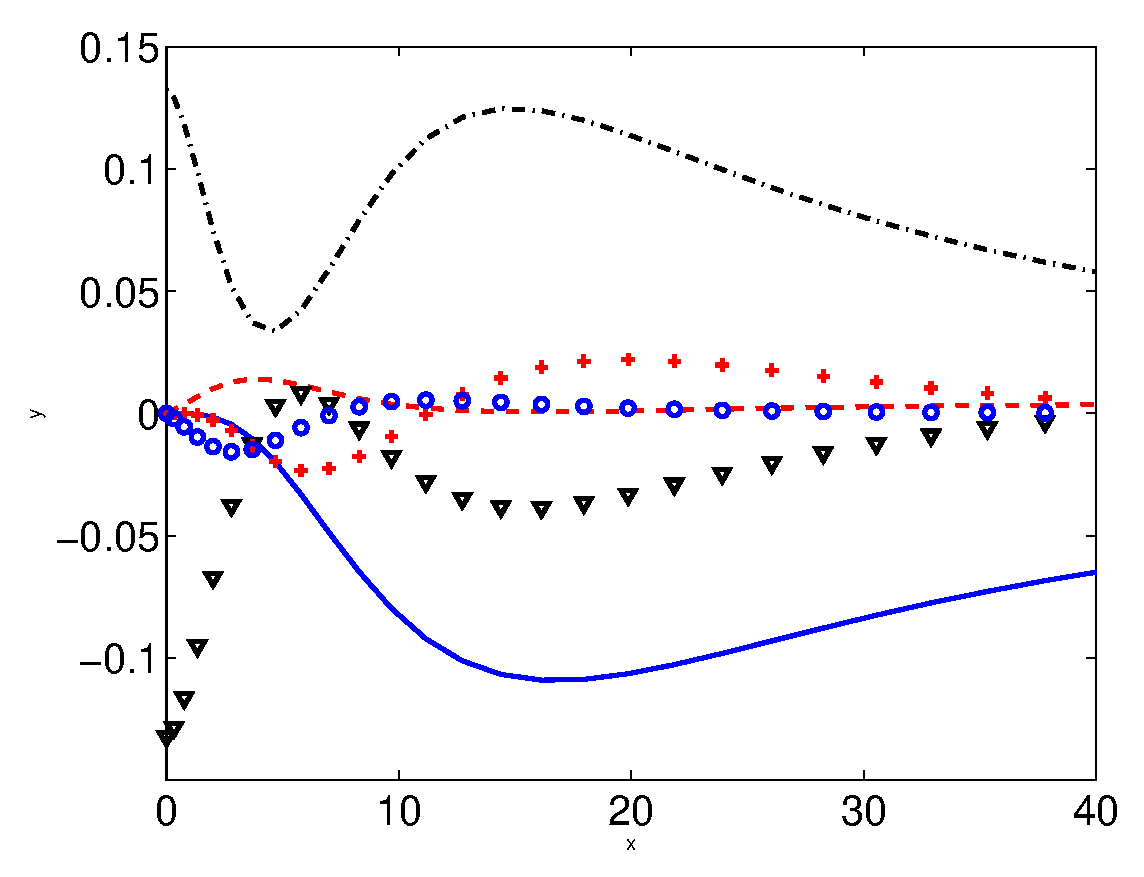
\includegraphics[width=7cm]{figur/balance_uv_zoom.eps}
\includegraphics[width=5.5cm]{figur/Energy_Spectrum_comp.png}
}
\end{minipage}%
\begin{minipage}[b]{0.5\textwidth}
%\psfrag{x}[r][1][1][0]{$x_2^+$}
%\psfrag{y}[r][1][1][0]{}
\subfigure[Outer region]{
\includegraphics[width=5.5cm]{figur/AA2016_Profiles_global_coords_comparison.jpg}
}
\end{minipage}
\caption{Channel flow at $Re_\tau=2000$. Terms in the $\overline{v'_1v'_2}$ equation scaled by $u_\tau^4/\nu$.
DNS data~\cite{hoyas:jimenez:06,hoyas:jimenez:web:data}.
\solidline: $P_{12}$;
\dashedline: $-\e_{12}$;
$\triangledown: -\D\overline{v'p'}/\D x_2$;
\dashdottedline: $\Pi_{12}$;
\textcolor{red}{$+$}: $-\D(\overline{v'_1v^{\prime 2}_2})/\D x_2$;
\textcolor{blue}{$\circ$}: $\nu \D^2\overline{v'_1v'_2}/\D x_2^2$.}
\label{uv_balance}
\end{figure}

If you want to learn more how to derive transport equations of turbulent quantities,
see~\cite{davidson:transport:06} which can be downloaded
\href{http://www.tfd.chalmers.se/~lada/allpapers.html}{here}\\
{\tt http://www.tfd.chalmers.se/\textasciitilde lada/allpapers.html}


\newpage
\appendix



\section{$\e-\delta$ identity}
%\e_{inm} \e_{mjk} i=1,n=2,j=1,k=2 => e_123e_312 =1
% \e_{min} \e_{mjk} i=1,n=2,j=1,k=2 => e_312e_312 =1
%
%\e_{inm} \e_{mjk} i=2,n=3,j=2,k=3 => e_231e_123 =1
% \e_{min} \e_{mjk} i=2,n=3,j=2,k=3 => e_123e_123 =1
%
%\e_{inm} \e_{mjk} i=2,n=1,j=2,k=1 => e_213e_321 =1
% \e_{min} \e_{mjk} i=2,n=1,j=2,k=1 => e_312e_321 =1
%
%\e_{inm} \e_{mjk} i=1,n=2,j=2,k=1 => e_123e_321 =-1
% \e_{min} \e_{mjk} i=1,n=2,j=2,k=1 => e_312e_321 =-1

The $\e-\delta$ identity reads

\begin{equation*}
 \e_{inm} \e_{mjk} = \e_{min} \e_{mjk} =  \e_{nmi} \e_{mjk} =\delta_{ij}\delta_{nk} - \delta_{ik}\delta_{nj}
\end{equation*}


In Table~\ref{eps-delta}  the components of the $\e-\delta$ identity are given.

\begin{table}[!t]
\begin{tabular}{|c|c|c|c|c|c|}\hline
$i$ & $n$ & $j$ & $k$ & $ \e_{inm} \e_{mjk}$ & $\delta_{ij}\delta_{nk} - \delta_{ik}\delta_{nj}$ \\ \hline
%
1   &  2  & 1   & 2   & $\e_{12m} \e_{m12}=\e_{123} \e_{312}= 1\cdot 1 = 1$ & $1-0=1$ \\
%
2   &  1  & 1   & 2   & $\e_{21m} \e_{m12}=\e_{213} \e_{312}= -1\cdot 1= - 1$ & $0 -1=-1$ \\
%
1   &  2  & 2   & 1   & $\e_{12m} \e_{m21}=\e_{123} \e_{321}= 1\cdot -1= - 1$ & $0-1=-1$ \\[0.3cm]
%
1   &  3  & 1   & 3   & $\e_{13m} \e_{m13}=\e_{132} \e_{213}= -1\cdot -1=  1$ & $1-0= 1$ \\
%
3   &  1  & 1   & 3   & $\e_{31m} \e_{m13}=\e_{312} \e_{213}= 1\cdot -1= - 1$ & $0-1=-1$ \\
%
1   &  3  & 3   & 1   & $\e_{13m} \e_{m31}=\e_{132} \e_{231}= -1\cdot 1= -1$ & $0-1=-1$ \\[0.3cm]
%
2   &  3  & 2   & 3   & $\e_{23m} \e_{m23}=\e_{231} \e_{123}= 1\cdot 1=  1$ & $1-0= 1$ \\
%
3   &  2  & 2   & 3   & $\e_{32m} \e_{m23}=\e_{321} \e_{123}=-1\cdot 1= -1$ & $0-1=-1$ \\
%
2   &  3  & 3   & 2   & $\e_{23m} \e_{m32}=\e_{231} \e_{132}= 1\cdot-1= -1$ & $0-1=-1$ \\ \hline
\end{tabular}
\caption{The components of the $\e-\delta$ identity which are non-zero.}
\label{eps-delta}
\end{table}



\bibliographystyle{unsrt}
\bibliography{bibfil}

\end{document}

